\documentclass[12pt,letterpaper]{book}

%%%%%%%%%%%%
% Includes %
%%%%%%%%%%%%
\usepackage[utf8]{inputenc}
\usepackage[margin=1 in]{geometry}
\usepackage{graphicx}
\usepackage{amsmath}
\usepackage{amsthm}
\usepackage{amsfonts}
\usepackage[justification=centering]{caption}
\usepackage{listings}
\usepackage[hidelinks]{hyperref}
\usepackage{parskip}

% Formatting
\renewcommand{\baselinestretch}{1.25}

% Theorems and other necessary structures
\theoremstyle{definition}
\newtheorem{definition}{Definition}[section] % Definition
\newtheorem{theorem}{Theorem}[section] % Big result
\newtheorem{corollary}{Corollary}[theorem] % Follows from a theorem
\newtheorem{lemma}[theorem]{Lemma} % Minor result
\newtheorem*{remark}{Remark}

% New commands
\newcommand{\R}{\mathbb{R}}
\newcommand{\N}{\mathbb{N}}
\newcommand{\Z}{\mathbb{Z}}

% Title information
\title{Computer Networks}
\author{2018A7PS0193P}

\begin{document}

\maketitle

\chapter{Networks}

\section{Introduction}

\begin{definition}
  A \textbf{network} is a shared infrastructure that allows users to communicate with each other.
\end{definition}

The basic building blocks of a network are \textbf{nodes} and \textbf{links}. Nodes may be hosts or forwarding nodes. The end hosts communicate with one another through the \textbf{core network}, consisting of forwarding nodes. These nodes are connected via links called \textbf{network edges}.

End hosts are physically connected to the core network via the \textbf{access network}. This consists of many parts, such as the ethernet switch, router, etc.

\section{Communication Models}

Networks could have multiple communication models:

\begin{itemize}
  \item \textbf{Client-Server model}: The client host requests, and receives the service from an always-on server. This server is also an end host, but has some special privileges.
  \item \textbf{Peer-peer model}: Here, there is minimal or no use of dedicates servers, as in BitTorrent. The clients directly communicate with one another.
\end{itemize}

\section{Core Network Models}

\subsection{Circuit Switching}

How is our core network made? One way to do this is via \textbf{circuit switching}. There are end-to-end resources reserved for a ``call", like on a telephone network. There is no sharing of resources. Call setup needs to be done as a preparatory step. Circuit switching generally can be implemented by two different methods:

\begin{itemize}
  \item \textbf{FDM}, which stands for Frequency Domain Multiplexing. The total frequency bandwidth is divided among the users, allowing them to send data simultaneously.
  \item \textbf{TDM}, which stands for Time Domain Multiplexing. Here the time is divided among the users (perhaps in a round robin fashion). As such, one user gets access to the entire bandwidth of the circuit, but only for a period in time.
\end{itemize}

\subsection{Packet Switching}

Another way is through \textbf{packet switching}, where data is sent over the net in discrete ``chunks", called packets. This is how it is done on the Internet. The host takes the application message, and breaks into packets of length $L$ bits. It then transmits packets into the access networks at transmission rate $R$, also called the bandwidth. Of course, this means that each packet faces a transmission delay of $L/R$.

Packet switching uses \textbf{store and forward}. The packets are stored at intermediate nodes before sending to the next node. The intermediate node checks for errors in the packets before transmitting, assuring the integrity of the packets.

Unlike circuit switching, packet switching does not provide guarantees of the bandwidth remaining constant. This is because it does not have any reserved end-to-end resources for a ``call''.

When using packet switching, there may be four sources of packet delay:

\begin{itemize}
  \item \textbf{Nodal processing} : The node performs error checking and checks the header for the destination of the packet.
  \item \textbf{Queueing} : When the arrival rate of the packets is faster than the sending rate, the node will keep the packets in a buffer queue. As such, there is a delay when the packet wait in the node queue.
  \item \textbf{Propagation} : This is the delay from propagation of the packets from a node to the next node, i.e., the outgoing delay. This depends on the medium of the wire, and is given by $d/s$, where $d$ is the length of the connection and $s$ is the speed.
  \item \textbf{Transmission} : This is the delay from transmission of packets into the link. If the transmission rate is $R$, the delay for one packet of length $L$ will be $L/R$.
\end{itemize}

\section{Performance of a Network}

The performance of a network can be measured by the following parameters:

\begin{itemize}
  \item Delay
  \item Packet loss : This is the number of packets lost when transmitting. Some applications, like streaming, might not care too much about this.
  \item Throughput : This is the amount of bits transferred in unit time. This is important in some applications, such as for file transfer.
\end{itemize}

\chapter{The Internet}

\section{Introduction}

The Internet is, in fact, a network of networks. The networks must be able to communicate despite using different applications running on different devices - i.e. it is heterogeneous.

As such, the Internet is full of different access ISP networks. How do end hosts on different access ISPs communicate with one another? Of course, if we directly connect them all, it would not be scalable as it would need $O(N^2)$ connections. We also cannot use a single global hub, since it would be difficult to find a single place to put it and connect the entire world.

Since a single global ISP cannot scale to connect the entire world, we use multiple global ISPs. These must be interconnected themselves. One way to do this is using \textbf{peering links}, which directly link two global ISPs. Another is to use \textbf{Internet Exchange Points}, called IXPs, to which multiple global ISPs can connect.

The Internet uses this system in a tiered manner - end hosts might connect to a regional ISP, which may then connect to a higher level country ISP, and so on.

Some corporations, like Google, have their own Content Distribution Networks (CDNs), and have their own network to bring services and content closer to users.

\section{Layered Network Model}

The Internet is based on a Layered Network Model known as \textbf{OSI}. Any device under OSI can have the following layers:

\begin{enumerate}
  \item Physical
  \item Data Link
  \item Network
  \item Transport
  \item Session
  \item Presentation
  \item Application
\end{enumerate}

Each of these layers depend on the one below (lower number) and export their services to the ones above (higher number).

The end hosts implement all 7 layers of the model. Those which implement the first 3 layers are called \textbf{routers} or Layer 3 devices. Routers are used to connect two different networks. Those which implement the first 2 layers are called \textbf{switches} or Layer 2 devices. They connect devices within a network, i.e., in Local Area Networks.

The Internet stack does not actually use all 7 layers - in fact it uses only 5. It removes the Presentation layer, which allows applications to interpret the meaning of data. It also removes the Session layer, which is used for synchronization, check pointing and recovery of data exchange. These functions are generally performed by the Application layer. This Internet stack is known as \textbf{TCP/IP model}.

In the context of the Internet, these layers perform the following functions:

\begin{enumerate}
  \item \textbf{Physical:} This layer delivers bits between the two endpoints of a link, e.g. copper, fiber, wireless, etc.
  \item \textbf{Data Link:} This layer delivers packets between two hosts in a local area network. These are bridges and switches.
  \item \textbf{Network:} This layer connects multiple networks, e.g. routers. This uses the Internet Protocol (IP).
  \item \textbf{Transport:} This layer does process-process data transfer. It may use a multitude of protocols, including TCP, UDP, etc.
  \item \textbf{Application:} This layer supports network applications. It may use FTP, SMTP, HTTP, etc.
\end{enumerate}

\section{IP Hourglass Architecture}

One way to imagine the Internet architecture is as a hourglass. The IP interconnects multiple existing networks, and hides the underlying technology from applications. This provides minimal functionality (has a ``narrow waist''). The trade-off of this approach is that there are no assumptions being made, and as such no guarantee that something works.

\chapter{The Application Layer}

\section{Network Applications}

A \textbf{Network application} is a program that runs on different end systems and communicates over a network. These are run only on the end hosts - core network devices do not run user application code.

The application architecture can run different application architectures:

\begin{itemize}
  \item \textbf{Client-Server}: The server is an ``always on'' host, which has a permanent IP address. To be able to scale, there are generally large data centers acting as a virtual server. The clients communicate with the server. Unlike the server, they may be intermittently connected, and may have a changing dynamic IP address. These clients never directly communicate with one another.
  \item \textbf{Peer to peer} : Here, there is not always on server. Instead the end hosts directly communicate with one another. The peers are connected and may change IP addresses dynamically.
  \item \textbf{Hybrid of client server and peer to peer} : This is the case in Instant Messaging and Skype. In instant messaging, the chatting between two users is P2P, but to get the IP addresses of a user's friends, a central server is needed.
\end{itemize}

Processes communicate within the same host using interprocess communication, but they must communicate with different hosts by exchanging messages.

\begin{definition}
  A \textbf{socket} is the interface between the application layer and the transport layer within the host.
\end{definition}

A process (a network application) send and receives messages using it's socket. This is a software entity, not a physical one.

To receive messages, each process must have some identifier. The IP address is not enough since it will only uniquely identify the host, but not the individual processes running on the host. So, we also use the port number to identify a process. For instance, an HTTP server would use port number 80, and a mail server would use port number 25.

\section{Application Transport Services}

What transport services does an application need? This changes from application to application. Here are some examples:

\begin{itemize}
  \item \textbf{Data Loss} : Depending on the application, it might be necessary that data transfer is 100\% reliable. For instance, in the case of file transfer, there must be no data loss, but some loss can be tolerated in the case of streaming.
  \item \textbf{Bandwidth} : Applications may also have bandwidth requirements. Streaming needs some minimum amount of bandwidth to work, but elastic applications like email and file transfer will make do with whatever bandwidth is available.
  \item \textbf{Timing} : Another parameter to consider is timing. Some applications, like games, require low delay, but for others this is unnecessary.
\end{itemize}

\section{HTTP}

The application layer for web pages is HTTP. A web page consists of objects, like HTML files, JPEG images, etc. Each of these objects is addressable by a URL. HTTP applications use TCP as it's transfer protocol.

\begin{enumerate}
  \item Client initiates the TCP connection on port 80. The time taken to establish this is called the \textbf{Round Trip Time} or RTT.
  \item Client sends a request to the server
  \item Server receives message through it's socket and sends the response.
  \item Server attempts to close the TCP connection. The client may refuse to do so if the client has not received the message.
  \item The client receives the message and closes the connection.
\end{enumerate}

It is important to remember that the time taken to send a file would be $2RTT + \text{File Transmission Time}$ - one RTT to establish connection, one RTT to send the first message and the time taken to send the file. Let us say the received file is an HTML file, which as 10 images embedded. Then, the client will request these images as well, by reopening the TCP connection and sending requests.

If at most one object is sent over a TCP connection, it is called \textbf{Non-persistent HTTP}. This was the case in HTTP version 1.0. In HTTP version 1.1, \textbf{Persistent HTTP} was introduced, which allows multiple objects to be sent over a single TCP connection between client and server. This could be done with or without a pipeline. If there is no pipeline, the client requests for each object, waits for the response, requests the next, and so on. To speed this up, we can use a pipeline and send requests for multiple objects one after another, while waiting for the response. The responses are always received in the same order in which they were sent.

\subsection{HTTP Requests}

A HTTP request message consists of:

\begin{itemize}
  \item A request line. It contains the method (POST,GET,HEAD), the URL being requested, and the HTTP version being used.
  \item Header lines. Each header line has the header field name and a value. An example of a header line can be \texttt{User-Agent: Firefox/3.6.10} or \texttt{Keep-Alive:115}.
  \item The body, which contains all the data of an entity
\end{itemize}

Each line is delimited by a carriage return character \textt{\textbackslash r} and a line feed character \texttt{\textbackslash n}.

The request methods could have the following meanings:

\begin{itemize}
  \item \texttt{GET} : This method is used to retrieve data from the server.
  \item \texttt{POST} : This is used to submit an entity to the server.
  \item \texttt{HEAD} : This asks the server for a response identical to a GET request, but without the response body.
  \item \texttt{PUT} : This is present in HTTP version 1.1. It uploads a file in entity body to the path specified in the URL field.
  \item \texttt{DELETE} : This is present in HTTP version 1.1. It deletes the file specified in the URL field.
\end{itemize}

\subsection{HTTP Responses}

A HTTP response message consists of:

\begin{itemize}
  \item A status line, which consists of the protocol, a status code and a status phrase. An example is \texttt{HTTP/1.1 200 OK}.
  \item Header lines, which are in the same format as in the request message. It could contain the time, the OS, etc.
  \item The body, which contains the requested data.
\end{itemize}

The HTTP response status codes are:

\begin{itemize}
  \item \texttt{200 OK} : Request succeeded, requested object later in this message.
  \item \texttt{301 Moved Permanently} : Requested object moved, new location specified in the Location header line.
  \item \texttt{400 Bad Request} : Request message not understood by the server.
  \item \texttt{404 Not Found} : Requested document not found on this server.
  \item \texttt{505 HTTP Version not supported} : The HTTP version used in the request is not supported by the server.
\end{itemize}

\subsection{States and HTTP}

HTTP is a stateless protocol - it does not save anything from it's previous actions. To save the state in HTTP, we use \textbf{cookies}. When a client sends a http request to the server, it will create an ID for the user and create an entry in the backend database. Now, when the server sends it's response, it will include a header line called \texttt{set-cookie}. From then onwards, the usual HTTP request message will send the cookie ID through a header line called \texttt{cookie}.

Hence, using cookies, we can save state with HTTP. This can be used to save user information and track them on other sites.

\subsection{Proxy Servers}

Proxy servers are also called web caches. Clients send their requests to a proxy server, which would forward it to the destination. The incoming responses are also forwarded to their respective clients. The proxy server can cache information, and hence answer requests itself to save time. This is especially useful in institutions when the content that users access has a large overlap.

One issue with this is that the cached data may turn stale. This problem is solved by the means of \textbf{Conditional GETs}. When a proxy server receives a response from the origin server, it will cache it before forwarding it to the end host. This response will have a header line called \texttt{Last-modified}, reflecting the time when that web page was last modified. Now the next time an end host requests that page, the proxy server will forward that GET request but with a header line \texttt{If-modified-since}, along with the date we got from the \texttt{Last-modified} header line. This effectively asks the server the question - has it been modified in the time since I last requested it? If it has, then the server removes the normal response, but otherwise it will get a \texttt{304 Not Modified} response. This response will not have any data, saving on bandwidth and time. This way, the proxy server is able to maintain the freshness of the cached data.

\subsection{HTTP/2 Protocol}

\begin{definition}
  A stream is a bidirectional sequence of text format frames sent over the HTTP/2 protocol exchanged between the server and client.
\end{definition}

HTTP/1 was capable of transmitting only one stream at a time. This made receiving large amount of media content inefficient and time consuming. HTTP/2 allows transmission of parallel multiplexed requests and responses. A binary framing layer is created, which allows the client and sever to disintegrate the HTTP payload into small independent and manageable interleaved sequence of frames. This information is then reassembled at the other end.

HTTP/2 also allows the server to send additional cacheable information to the client that isn't requested but is anticipated to be needed in future requests. This mechanism saves a RTT and reduces network latency. This is called \textbf{Server PUSH}.

\section{Domain Name System}

When a client requests the URL, it must obtain the IP address of the destination host to send the request to. The \textbf{Domain Name System} maps the name people use to locate a website to the IP address that a computer uses to locate a website.

The DNS is formed by a distributed hierarchical database. The 13 \textbf{root DNS} servers contain reference to the \textbf{top level domain} servers, like the .com servers, the .org servers, etc. These then contain references to the \textbf{authoritative servers}, which are maintained by organizations with publicly accessible hosts to map the hostnames to IP addresses. Examples of this would be servers for yahoo.com or google.com.

One issue we would face is that since we would need to traverse the hierarchy recursively to query a host, it can take a long time to process a DNS query. In practice, instead of traversing the tree on a direct path, the local DNS server would first get information about the TLD DNS server from the root server, and then contact the TLD server directly, instead of letting the root DNS server do this. This is done recursively, contacting lower and lower levels in the hierarchy directly from the local DNS server and getting the IP of the next level.

DNS responses are generally cached to improve the delay performance and to reduce the number of DNS messages.

DNS provides the following services:

\begin{itemize}
  \item \textbf{Host name to IP address mapping} : Websites are generally identified by their hostname. DNS provides a mapping of hostnames to IP addresses, which is what the end host needs to connect to the server.
  \item \textbf{Host aliasing} : Sometimes, hosts have complicated names, and hence can have one or more alias names. The non-alias hostname is called the canonical hostname. DNS can also be used to find the canonical hostname for a supplied alias.
  \item \textbf{Mail server aliasing} : It is highly desirable that an email address is easy to remember. The hostname of the Gmail mail server may be very complicated. DNS can be invoked by a mail application to obtain the canonical hostname for the given email address alias.
  \item \textbf{Load distribution} : DNS is used to perform load distribution in the case of replicated servers, where one canonical hostname is associated with multiple IP address. The DNS server rotates these IP addresses upon every query to ensure load management.
\end{itemize}

The DNS servers store the necessary information in the form of resource records(RR). They are in the format \texttt{(name, value, type, ttl)}. Here \texttt{ttl} stands for ``time to live'', which tells the DNS resolver how long to cache a query before requesting a new one. The values of the other fields depends on the type of the resource record. There are four types of resource records, depending on the \texttt{type}:

\begin{itemize}
  \item \texttt{type=A} : \texttt{name} refers to the host name, and \texttt{value} refers to the IP address.
  \item \texttt{type=NS} : \texttt{name} is the domain name, and \texttt{value} is the host name of authoritative name server for this domain.
  \item \texttt{type=CNAME} : \texttt{name} is the alias name for some canonical name, \texttt{value} is the canonical name.
\item \texttt{type=MX} : \texttt{value} is the name of the mail server associated with the \texttt{name}.
\end{itemize}

To insert a record into DNS, a newly created domain name should be first registered at a registrar.

\section{File Transfer Protocol}

This protocol is used to transfer file from client to client. It uses the TCP protocol, since it must be reliable and error free.

In a typical session, FTP will use two connections - a control connection and a data connections. The control connection, which is generally established on port 21, is the primary connection and is used to send commands back and forth between the client and the server. The data connection, established on port 20, is used solely to transfer the requested data. It stays open until the transfer is complete. Since FTP uses two parallel TCP connections to transfer a file, it is said to send it's control information \textbf{out of band}. This is in contrast to HTTP, which works \textbf{in band}.

Unlike HTTP, the FTP server must maintain the state of the user. In particular, the server must associate the control connection with a specific user account and keep track of the user's current directory as the user wanders about the remote directory tree. This unfortunately constrains the total number of sessions that FTP can can maintain simultaneously.

Some FTP commands are:

\begin{itemize}
  \item \texttt{USER username}
  \item \texttt{PASS password}
  \item \texttt{LIST} returns list of file in current directory
  \item \texttt{RETR filename} retrieves file
  \item \texttt{STOR filename} stores file onto remote host
\end{itemize}

These commands can give return codes and phrases as in HTTP:

\begin{itemize}
  \item \texttt{331 Username OK, password required}
  \item \texttt{125 data connection already open; transfer starting}
  \item \texttt{425 can't open data connection}
  \item \texttt{452 Error writing to file}
\end{itemize}

\section{eMail}

e-Mail consists of three major components

\begin{itemize}
  \item User agents, e.g. Outlook, mutt
  \item Mail servers, Contains incoming messages for user
  \item Simple Mail Transfer Protocol (STMP)
\end{itemize}

A user creates a mail and sends it to their mail server using the user agent. The sender's mail server will forward this mail to the recipient's mail server over a TCP connection on port 25. The recipient's user agent will then try to access this mail from the server. The protocol used in this case is called \textbf{Mail Access Protocol}, like IMAP or POP3. Everywhere else in this process, we use SMTP. We cannot use SMTP for the recipient to access the mail, since SMTP is a push-based protocol, not a pull based protocol.

POP3 is the Post Office Protocol. It allows the user to download and keep the mails. The user can create folders and move the messages into them locally. It is stateless across sessions.

A more feature-rich protocol is IMAP or the Internet Mail Access Protocol. It allows the user to create remote folders and maintains user state information across sessions, It also permits a user agent to obtain components of messages, which is ideal for low bandwidth connections.

The user agent could be web-based, like in Hotmail or Gmail. Now, the transfer of the message from the sender to the mail server happens over HTTP. The access of mails by the receiver is also done over HTTP.

\section{Peer To Peer Architecture}

As mentioned before, there is no always-on server in peer-to-peer architectures. The end hosts directly communicate, and the peers are intermittently connected.

Let us say we want to send $N$ file copies of size $F$. In a client-server system, ignoring the delays, the time taken to send to a server would be $NF/u_s$, where $u_s$ is the upload rate. Each client must download a file copy, and it the slowest download speed is $d_{min}$, then the slowest download time would be $F/d_{min}$. So, the minimum time to distribute to the $N$ clients would be:
\[D_{c-s} \geq \max(NF/u_s,F/d_{min})\]
In the case of P2P system, at least one copy must be uploaded, taking time $F/u_s$. Each client must download a file copy, with the slowest download time once again being $F/d_{min}$. Unlike in the client-server scheme, as the file download gets completed on peers, the number of possible ``providers'' increases. As this happens the maximum upload rate increases, up till $u_s +\sum u_i$. So, the time needed is:
\[D_{P2P} \geq \max(F/u_s,F/d_{min},NF/(u_s+ \sum u_i))\]

In BitTorrent, a peer-to-peer application, the file is divided into chunks, typically 256 KB in size. There are trackers that track peers participating in a torrent. A new peer joins a torrent and registers with the tracker to get a list of peers, and connects to some subset of them. While torrenting, a group of peers exchange chunks of a particular file. At any given time, each peer will have a subset of the chunks, and asks its neighbours for a list of which chunks they have. The peer will then take a call on which chunks it should request from the neighbour, and to which of its neighbours it should send requested chunks. Ideally, the peer would request and send the most scarce chunks.

One P2P protocol is \textbf{Napster}. Here, we have a central database where information is available, and the peers contact it for the necessary information. However, if the database is down then the peer-to-peer application cannot run.

Another P2P protocol is \textbf{Gnutella}. Unlike Napster, it is a completely decentralized protocol. On startup, an end host finds at least one other node to connect to. It then queries this node for more nodes to connect to, until it reaches some quota. Due to the completely decentralized network, this protocol is not scalable - searching takes time exponential in the number of nodes, and often end hosts are only connected intermittently.

Yet another P2P protocol is \textbf{Kazaa}, which is the basis for Skype. Kazaa is also a decentralized system. The users are divided into two groups - supernodes and ordinary nodes. Supernodes are powerful computers that act like traffic hubs, processing data requests from ordinary nodes.

\section{Distributed Databases}

Distributed databases are a common application of the P2P framework. In a distributed database, each peer holds a small subset of the total (key,value) pairs. Any peer can query the distributed database with a particular key. The distributed DB locates the peers that have the corresponding (key,value) pairs and return it to the querying peer. Any peer can insert a new (key,value) pair into the database.

A non-scalable way of doing this is as a distributed hash table. The key,value pairs are randomly scattered across all the peers. They maintain a list of the IP addresses of all the peers, and send their queries to all these peers. Those who contain the required (key,value) pairs respond with the matching pairs. This is, as mentioned before, not scalable since all peers must be queried.

Instead we may implement this with the \textbf{Circular DHT}  protocol. A hash function assigns each node and key an $m$ bit identifier using a base hash function such as SHA-1. The node's ID could be a hash of the port and the IP address, while the key's ID can be a hash of the original key. Since there is a finite number of hashes, these ID values will lie on an imaginary circle, ranging values from $0$ to $2^{m-1}$. We now assign (key,value) pairs to the peer that has the next closest node ID to the pair's key ID.

One protocol that uses this concept is the \textbf{Chord protocol}. Every node keeps track of 2 pointers - the predecessor, a pointer to the previous node on the ID circle, and the successor, a pointer to the next node on the ID circle. When doing a lookup operation, a node will check whether the key's ID is between the ID of the node and it's successor. In this case, it will know that the key is present in the successor. If not, the query is forwarded to the successor, and the same operation is done recursively. The number of messages is $O(n)$, where $n$ is the number of nodes. So, this is not scalable.

A scalable way to do this is that each node $n$ contains a routing table with up to $m$ entries ($m$ is the number of bits), known as a \textbf{finger table}. The $i^{th}$ entry in the table at node $n$ contains the first node $s$ that succeeds $n$ by at least $2^{i-1}$, i.e. $s = succ(n+2^{i-1})$. $s$ is called the \textbf{ $i^{th}$ finger} of node $n$. With this information, we can jump to the furthest successor that precedes the key ID.

In a P2P system, peers can connect and disconnect without warning. Thus, when designing the DHT, we have to be able to maintain the correct successor pointers. To achieve this, each node maintains a successor list of its $r$ nearest successors on the ring. If node $n$ notices that it's successor has failed, then it will replace it with the next entry on the list. This checking needs to be done often based on the frequency of nodes leaving and joining.

\section{Socket Programming}

A socket is created whenever we desire communication between two applications running on different machines. In UNIX, this is merely another file descriptor. The socket is created with the \texttt{socket(domain, type, protocol)} system call. The domain contains the address family, the type specifies the semantics of communication, e.g. SOCK\_STREAM for stream sockets, SOCK\_DGRAM for datagram sockets, etc. The protocol specifies whether it is UDP (IPPROTO\_UDP) or TCP(IPPROTO\_TCP).

To establish a connection, the client does the following:

\begin{enumerate}
  \item Create a socket
  \item Connect the socket to the address of the server
  \item Send/Receive data
  \item Close the socket
\end{enumerate}

To establish a connection, the server does the following:

\begin{enumerate}
  \item Create a socket
  \item Bind the socket to the port number known to all clients.
  \item Listen for the connection request
  \item Accept the connection request
  \item Send/receive data
\end{enumerate}

The socket address is stored in the following struct

\begin{lstlisting}[language=c]
  struct sockaddrs {
    unsigned short sa_family; // address family, AF_xxx or PF_xxx
    char sa_data[14]; // 14 bytes protocol address
  };
\end{lstlisting}

AF stands for address family and PF stands for protocol family. For IPv4 internet protocols, we use AF_INET.

There is also the following construct, that contains information about the address family, port number, internet address and the size of the struct sockaddr.

\begin{lstlisting}[language=c]
struct sockaddr_in{
  short int sin_family; // Address family
  unsigned short int sin_port // Port number
  struct in_addr sin_addr; // Internet address
  unsigned char sin_zero[8]; // same size as struct sockaddr
}
\end{lstlisting}

Some systems are little endian, while others could be big endian. To communicate between these two systems, a standard has been defined for the data representation in the network called \textbf{Network Byte Order}, which is big endian. The system calls that help us convert a short/long from host byte order to NBO and vice versa are:

\begin{itemize}
  \item \texttt{htons()} : Host to Network short
  \item \texttt{htonl()} : Host to Network long
  \item \texttt{ntohs()} : Network to Host short
  \item \texttt{ntohl()} : Network to Host long
\end{itemize}

\chapter{Transport Layer}

\section{Introduction}

The transport layer is responsible for logical communication between the hosts, unlike the network layer which is responsible for logical communication between processes. Since the transport layer works on top of the network layer, it is constrained by the underlying network layer protocol. However, in some cases it can offer services even when the network layer doesn't offer it.

The transport layer provides two protocols - UDP, an unreliable connectionless service, and TCP, a reliable, connection oriented service. The transport layer works with transport layer packets called \textbf{segments}.

\section{Multiplexing and Other Functions}

The transport layer multiplexes messages at sending time by handling data from multiple sockets and adding a transport header for each message. It is also responsible for demultiplexing the received messages by using the header information to deliver the received messages to the correct sockets. These are the only two services UDP provides, but TCP provides some additional services. As mentioned before, it also proved reliable data transfer. Besides this, it provides what is called congestion control. TCP congestion control prevents any one TCP connection from swamping links and routers between hosts with excess traffic, and tries to give every connection an equal share of traffic.

In \textbf{connectionless multiplexing}, as seen in UDP, the sockets are identified by a port number. So to perform multiplexing, the segments must contain information of a source port number and a destination port number.This information is passed from the sender's transport layer to it's network layer, which encloses it within a \textbf{datagram}  (network layer packet). This datagram will now also have information about the sender's IP address and the destination IP address. Finally, when this message reaches the destination, that host checks the destination port number and redirects the message to that port. The source port number seems unnecessary, but acts as a ``return address'' for the application to use to communicate.

As such, a UDP segment has the following content:

\begin{itemize}
  \item 16 bit Source port number
  \item 16 bit Destination port number
  \item 16 bit length
  \item 16 bit checksum, which is used to detect errors. This is calculated by treating the segment contents as a sequence of 16-bit integers, and summing them all. The one's complement of the sum is put in this field.
  \item The rest is the application data
\end{itemize}

TCP uses \textbf{connection oriented multiplexing}. Unlike a UDP socket, a TCP socket is identified by a 4-tuple of (source IP address, source port number, destination IP address, destination port number). Thus, when a TCP segment arrives from the network to a host, the host uses all four values to demultiplex the segment to the appropriate socket. In contrast with UDP, two arriving TCP segments with different source IP addresses or source port numbers will be directed to two different sockets.

Knowing that UDP is unreliable, one might wonder why we use UDP at all. Some reasons are as follows:
\begin{itemize}
  \item No connection establishment, which would add delay
  \item It is simple, since there is no connection state to maintain at the sender and the receiver end
  \item It has a small header size
  \item It has no congestion control. While this is undesirable in some cases, it means that UDP can run as fast as desired.
\end{itemize}

\section{Designing a Reliable Data Transfer}

Let us assume that the underlying channel is perfectly reliable. Then, let us design a protocol called \texttt{rdt1.0}. We diagrammatically show this as two Finite State Machines - one for the sender, and another for the receiver.

\begin{figure}[htpb]
  \centering
  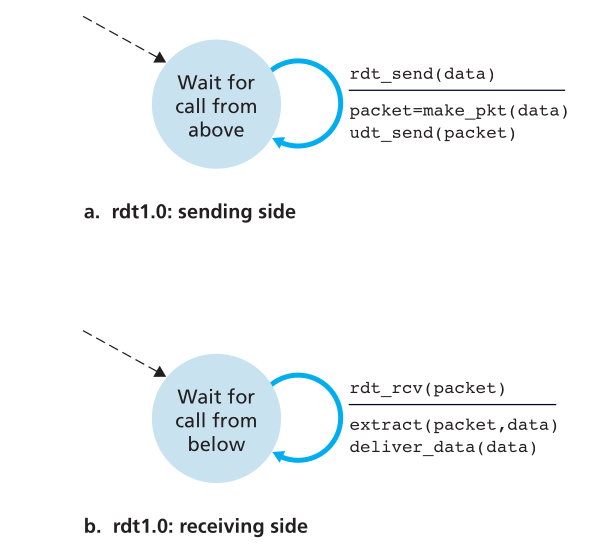
\includegraphics[width=0.8\linewidth]{./assets/rdt1_fsm.png}
  \caption{FSM for rdt1.0}%
  \label{fig:}
\end{figure}

As we can see in Fig 1, sender simply sends data into the underlying channel, and the receiver simply reads from the underlying channel.

What if our underlying channel has some bit errors? Then the packet may have some flipped bits! For this we design our second protocol, \texttt{rdt2.0}. For this, we can use the checksum to detect the bit errors. If there were no bit errors, the receiver will return an \textbf{acknowledgement} (ACK), explicitly telling the sender that the packet is OK. If not, the receiver will return a \textbf{negative acknowledgement} (NAK), saying that the packet had errors. In this case, the sender will retransmit packets. The FSM for the same is in Fig 2.

\begin{figure}[htpb]
  \centering
  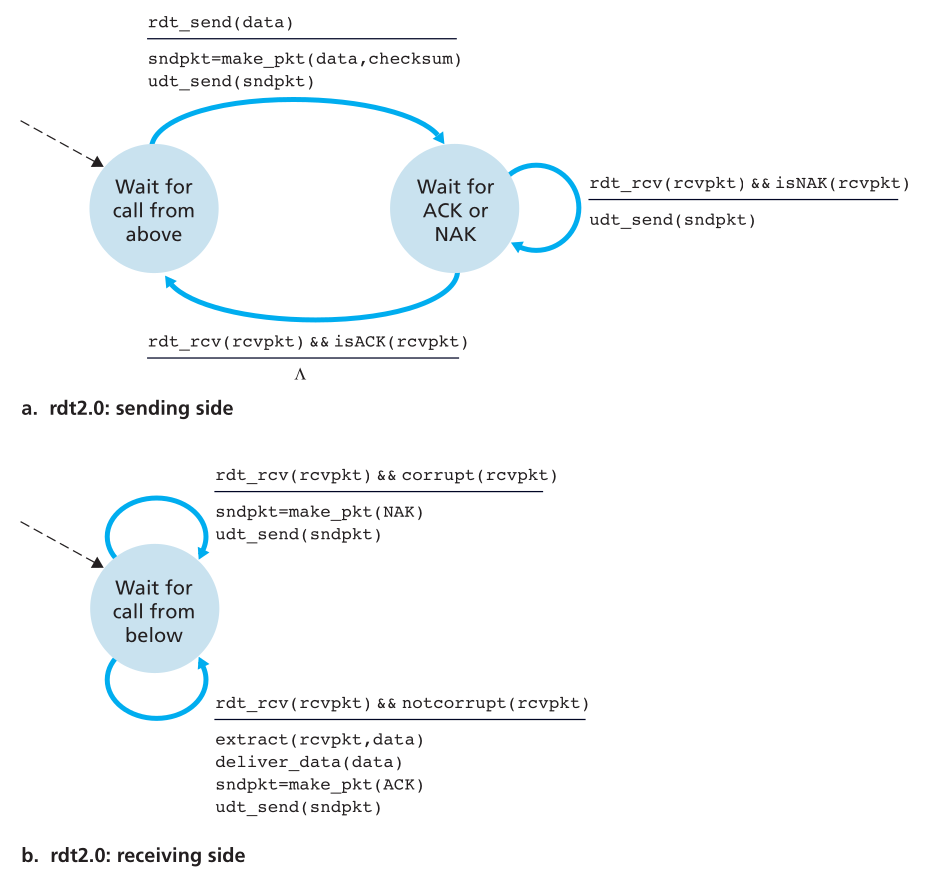
\includegraphics[width=0.8\linewidth]{./assets/rdt2_fsm.png}
  \caption{FSM for rdt2.0}%
  \label{fig:}
\end{figure}

However, this has a fatal flaw. What if ACK/NAK is corrupted? One way to handle this is to be safe, and send the packet again if the ACK/NAK is corrupted. But this creates a new problem of handling duplicate packets, where the receiver is unsure if this is new information of old data. To fix this, the sender adds a sequence number to each packet. The receiver checks this to decide which packet to discard.  For instance, say $A$ sends a packet with sequence number 0 to $B$. $B$ sends back an ACK, but it gets corrupted on the way back. Then, $A$ will send the packet again with the same sequence number. However, $B$ will know this is a duplicate, since it has the same sequence number as the last packet. In this mechanism (called a stop and wait mechanism), we need only 1 bit for the sequence numbers.

This creates a new protocol - \texttt{rdt2.1}. The FSMs are as in Fig 3 and 4.

\begin{figure}[htpb]
  \centering
  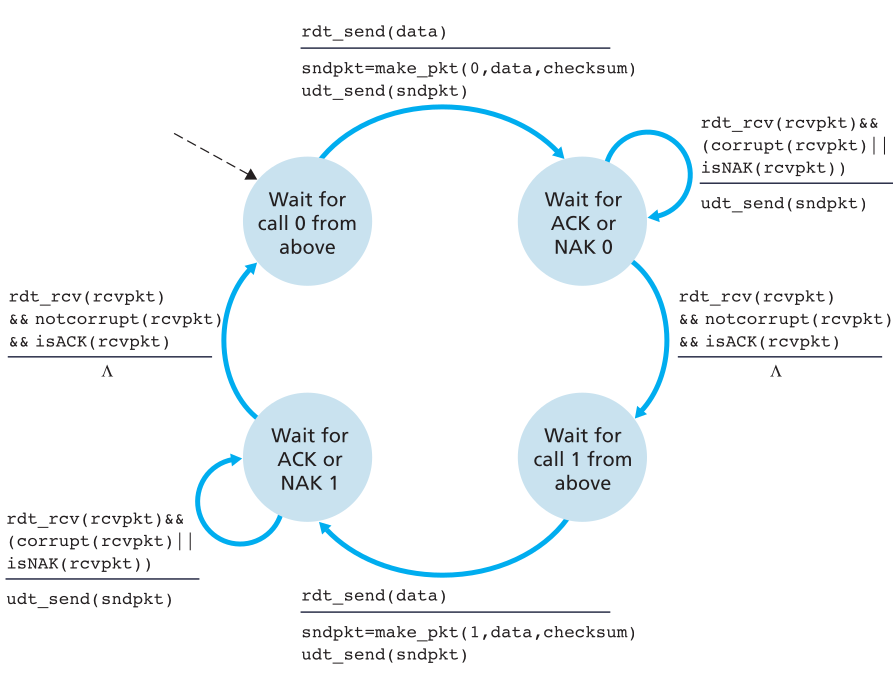
\includegraphics[width=0.8\linewidth]{./assets/rdt2-1_sender.png}
  \caption{rdt2.1 Sender}%
  \label{fig:name}
\end{figure}

\begin{figure}[htpb]
  \centering
  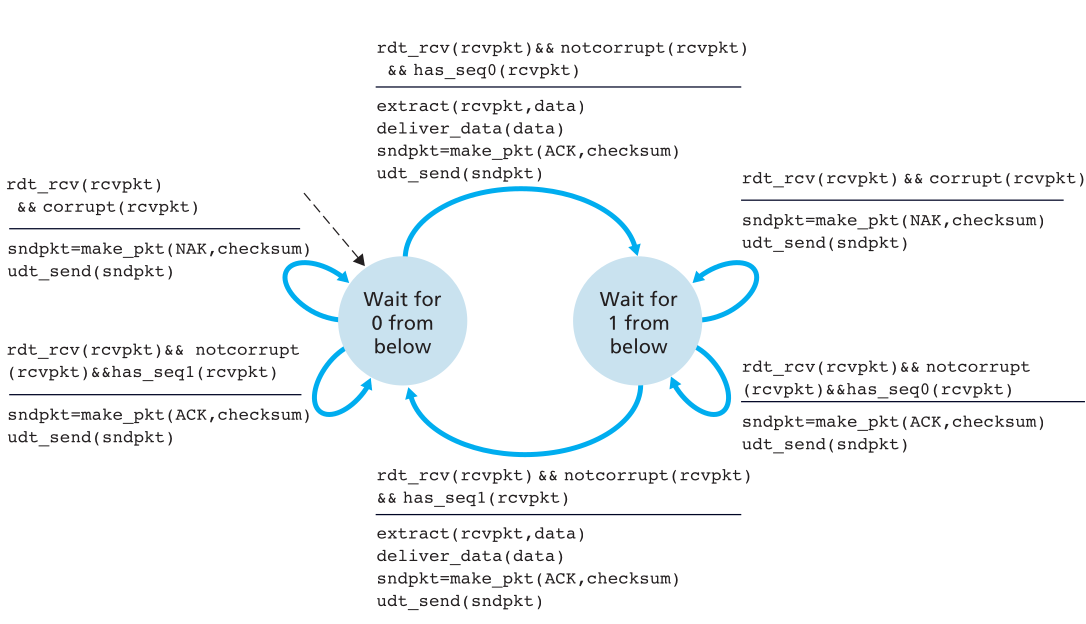
\includegraphics[width=0.8\linewidth]{./assets/rdt2-1_rcvr.png}
  \caption{rdt2.1 Receiver}%
  \label{fig:./assets}
\end{figure}

We can remove the need for NAKs by sending ACK for the last correctly received packet instead. If a sender receives two ACKs for the same packet, it knows that the receiver did not correctly receive the packet following the packet that is being ACKed twice. This new protocol is \texttt{rdt2.2}.

Let us now assume that the underlying channel could also lose packets entirely. \texttt{rdt2.2} gives us the base to start from, but we need to handle the lost packets. We put the burden of detecting and recovering from lost packets on the sender. Suppose that the sender transmits a data packet and either that packet or the receiver's ACK of that packet gets lost. If the sender is willing to wait long enough so that it is certain that a packet has been lost, it can retransmit the data packet. But how long is long enough? We could choose the worst case, but that is difficult to approximate and may be too slow. So we just choose some time value that packet loss is very likely, but not guaranteed to have happened.

Even in this case, we could have duplicate data packets, since the ACK could just have been received very late due to some delays, even if the packet was not lost. Luckily, rdt2.2 can already handle this case using sequence numbers. Thus, we now have \texttt{rdt3.0}. Since the sequence numbers are either 0 or 1, it's also called a alternating bit protocol. In Fig 5 we can see the FSM for the sender in \texttt{rdt3.0}.

\begin{figure}[htpb]
  \centering
  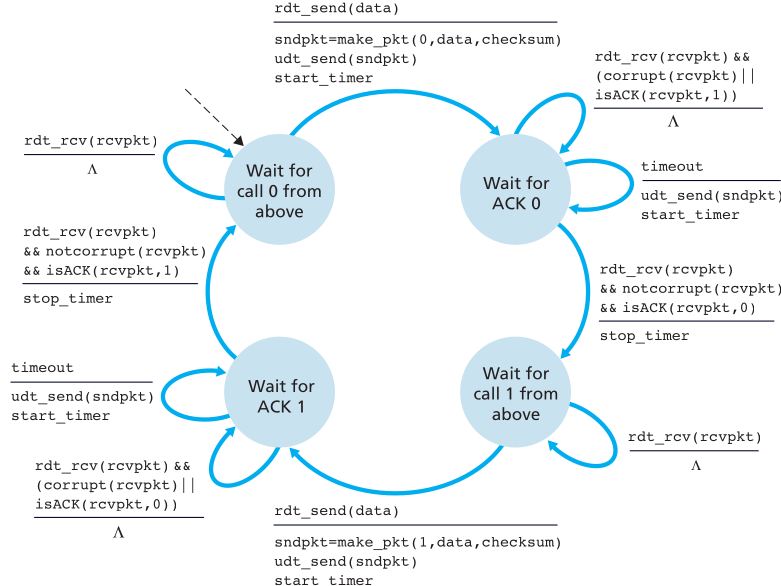
\includegraphics[width=0.8\linewidth]{./assets/rdt3_fsm.png}
  \caption{rdt3.0 sender}%
  \label{fig:./assets}
\end{figure}

\texttt{rdt3.0} is good, but it has it's own issue. Let us define \textbf{utilization} of the sender as the fraction of time the sender is actually busy sending bits into the channel. If we are sending $L$ bits per packet, and $R$ is the rate of transmission, the sender will spend $\frac{L}{R}$ time sending bits. However, the time taken to receive the acknowledgements for the packet will be $RTT$. So,
\[U = \frac{L/R}{RTT+L/R}\]
This $U$, if calculated, is generally found to be dismal in the case of \texttt{rdt3.0}. Instead, we use a pipelined protocol.

\begin{remark}
  As an aside, we can also define the utilization as the fraction of the bandwidth being used. So if we take $T$ time to send $L$ bits, the amount of bandwidth being used is $L/T$. This is also called the effective bandwidth or the throughput. As such, we can define the utilization as:
\[U = \frac{Throughput}{R}\]
where $R$ is the total bandwidth of the connection.
\end{remark}

In a pipelined protocol, the sender may send multiple packets despite not having received the ACK. If one sends $n$ packets at once, we can increase the utilization by a factor of $n$. However, this comes with multiple consequences:

\begin{itemize}
  \item The range of sequence numbers must be increased.
  \item The sender and receiver sides of the protocols need to buffer more than one packet.
\end{itemize}

We can have two pipeline protocols - Go-Back-N (GBN) or Selective Repeat (SR).

In a GBN protocol, the sender is  allowed to send multiple packets without waiting for an ACK, but it is constrained to some maximum allowable number $N$. Let us define \texttt{base} as the sequence number of the oldest unacknowledged packet and \texttt{nextseqsum} to be the smallest unused sequence number. Then, we have four intervals:

\begin{itemize}
  \item \texttt{[0,base-1]} : corresponds to the packets that have already been transmitted and acknowledged.
  \item \texttt{[base,nextseqsum-1]} corresponds to packets that have been sent but not acknowledged.
  \item \texttt{[nextseqnum,base+N-1]} can be used for packets that can be sent immediately
  \item \texttt{base+N} and greater cannot be used until an unacknowledged packet currently in the pipeline has been acknowledged
\end{itemize}

So, the window of permissible numbers transmitted but not yet acknowledged packets can be viewed as a sliding window of size $N$.

In the GBN protocol, an ACK for a packet with sequence number $n$ will be taken as cumulative acknowledgement, indicating that all packets with a sequence number up to and including $n$ have been correctly received at the receiver. Just like in \texttt{rdt3.0}, a timer is used to recover from lost data or acknowledgement protocols. If a timeout occurs, the sender resends all packets that have been previously sent but not acknowledged.

In GBN, the receiver also discards out of order packets. This means that the receiver need not buffer out of order packets. The receiver hence maintains the sequence number of the next in order packet, called \texttt{expectedseqnum}. If an out of order packet is received, it is discarded. This is equivalent to saying that GBN has a receiver's window of size 1.

GBN has it's downsides:

\begin{itemize}
  \item If window size and bandwidth-delay product are both large, many packets can be in the pipeline.
  \item A single packet error can cause retransmission of many packets
\end{itemize}

Selective Repeat avoids unnecessary retransmissions by having the sender retransmit only the packets that it suspects were received in error at the receiver. This means that the receiver must individually acknowledge the correctly received packets. Like in GBN, a window of size $N$ will limit the number of outstanding unacknowledged packets in the pipeline, but unlike GBN, the sender will have already received ACK for some of the packets in the window. Of course, the window will not move past any unacknowledged packets until they have been acknowledged.

The SR receiver will also ACK packets even if they are received out of order. Out of order packets are buffered until any missing packets are received, at which point they are delivered to the upper layer.

In SR protocols, the sender and receiver do not always have the same windows. This lack of synchronization can result in issues when we deal with windows of finite sizes. It is possible to show that the window size should ideally be less than or equal to half the size of the sequence number space.

\section{TCP}

\subsection{Introduction}

Just like the protocols we have designed before, TCP is a point to point protocol that allows bidirectional flow of data. It provides a reliable in-order byte stream - this means there are no message boundaries. It is a pipeline protocol, where the window size is set by the congestion and flow control in TCP. Unlike UDP, it is connection oriented.

\subsection{The TCP Segment}

The important fields in a TCP segment are:

\begin{itemize}
  \item 16 bit Source port number
  \item 16 bit Destination Port number
  \item 32 bit sequence number, indicating the sequence number of the first byte.
  \item 32 bit acknowledgement number. If a 200 byte message is sent with sequence number 100, then the receiver will return a segment with an acknowledgement number of 300, indicating that sequence numbers up to 299 has been received, and we expect to receive sequence number 300 next.
  \item 4 bit header length. This indicates that the header length is not always fixed, since the options in the header can be of variable length
  \item Urgent data flag. It is generally unused.
  \item Valid acknowledgement bit, indicating whether or not the acknowledgement number is to be considered. If it is 0, then the acknowledgement bit can be a garbage number.
  \item PSH flag, telling to push the data now
  \item RST,SYN,FIN flags, used to setup and destroy connections.
  \item 16 bit receive window, which is the number of bytes that the receiver is willing to accept. This is used for flow control.
  \item 16 bit checksum, used to detect bit errors during transmission.
\end{itemize}

\subsection{Handshaking}

Before exchanging data, the sender and receiver must do a handshake, agreeing on the parameters of the connection. One way to do this is a 2 way handshake - the sender ``asks'' for a connection with the receiver, and the receiver responds with a ``yes'' or ``no''. If it is a ``yes'', then we can establish it. However, this is not actually enough. Since the underlying channel is not reliable, the reply (yes or no) could be dropped, and the receiver is unsure if the sender has received the reply. Hence, a third segment is sent, confirming the receipt of the ``yes'' or ``no''. This is called 3-way handshaking. Formally, the steps are as follows:

\begin{enumerate}
  \item The client chooses an initial sequence number $x$ and sends a TCP SYN message. This message has it's SYN flag set to one. The segment has no application layer data - it is just used to establish a connection. After doing this, the client enters the SYNSENT state.
  \item On receiving the SYN message, the server enters the SYN RCVD state. The server chooses an initial sequence number $y$ and sends a TCP SYNACK message. This has it's SYN and ACK flags set to 1. The acknowledge number will be equal to $x+1$, indicating the server expects to receive a sequence number $x+1$ next.
  \item The client on receiving SYNACK believes the server is live, and enters the ESTAB state. It now sends an ACK for the SYNACK, so the ACK bit is set to 1 and the acknowledgement number is $y+1$. This segment may contain application data. If it does, this is called \textbf{piggybacking}.
  \item The server receives ACK and believes the client is live. The connection has been established, and the server also enters the ESTAB state.
\end{enumerate}

\subsection{Sending Data}

When sending data from the client to the server, the client passes a stream of data through the socket, into the hands of the transport layer and the TCP protocol. TCP directs this data to the send buffer of the client, and when possible, will forward chunks of data from it to the network later. The maximum amount of data that can be placed in a segment is called the \textbf{maximum segment size} or MSS. This is decided by considering the length of the largest link-layer packet that can be sent, called the \textbf{maximum transmission unit} or MTU. The MSS is a multiple of 8 bytes chosen such that the TCP segment and the TCP/IP header length will fit into a single link layer frame. This stream of data is received by the server in the receive buffer and duly processed. This process happens on both sides of the connection, since TCP is bidirectional.

To prevent the sender from overflowing the receiver's buffer, TCP provides \textbf{flow control}. The sender maintains a variable called a \textbf{receive window}, used to give the sender an idea of how much free buffer space is available to the receiver. Let \texttt{LastByteRead} be the number of last byte in the data stream read from the buffer by the application process in B, and \texttt{LastByteRvcd} be the number of the last byte in the data stream that has arrived from the network and has been placed in the receive buffer at B. Since TCP must not overflow the allocated buffer, we must have:

\texttt{LastByteRvcd - LastByteRead <= RcvBuffer}

The receive window denoted by \textt{rwnd} is then the amount of spare room in the buffer, given by

\texttt{rwnd = RcvBuffer - (LastByteRvcd - LastByteRead)}

While the receiver B keeps track of \texttt{rwnd}, A keeps track of two variables - \texttt{LastByteSent} and \texttt{LastByteAcked}. \texttt{LastByteSent - LastByteAcked} is obviously the amount of unacknowledged data A has sent into the connection. A makes sure this amount is less than the value of \texttt{rwnd} to ensure that the receive buffer is not being overflowed.

If \texttt{rwnd} is ever 0, A will keep sending segments with one data byte to B to check whether space has freed up in the receive buffer.

\subsection{Closing The Connection}
When closing the connection, the following steps are taken:

\begin{enumerate}
  \item The client sends a closing request using \texttt{clientsocket.close()}. This segment will have a sequence number of $x$ and have the FIN flag set. The client will no longer send data, but will be able to receive data. The client is said to be in the FIN\_WAIT\_1 state.
  \item The server responds with an ACK. The server enters the CLOSE\_WAIT state, while the client (on reception) enters the FIN\_WAIT\_2 state. The client is now waiting for the server to close.
  \item The server will enter the LAST\_ACK state, and sends it's own closing segment, where FIN bit is set to 1. The client will acknowledge this with an ACK, which will put the server in a CLOSED state.
  \item The client now enters a TIMED\_WAIT state, where it will wait for some predetermined time (say 30 seconds) before considering the connection closed. This allows the client time to resend the final acknowledgement in case the ACK is lost.
\end{enumerate}

From the above discussion, it is clear that unlike the connection establishment, connection closure is a 4-way handshake.

\subsection{Timeouts}

TCP, just like the \texttt{rdt} protocol, uses a timeout mechanism to recover from lost packets. How do  we decide the length of the timeout interval? It must be larger than the RTT, but how do we estimate it?

To choose the timeout interval, the sender first finds the RTT from the last segment sent, called the $SampleRTT$. TCP only does this for a single transmitted (but yet unacknowledged) segment at a time, and only those which have been transmitted only once. This value will obviously fluctuate with time, and hence TCP maintains an exponential weighted moving average called $EstimatedRTT$ calculated by the formula:
\[EstimatedRTT = (1-\alpha) EstimatedRTT + \alpha SampleRTT\]
We also estimate the deviation of $SampleRTT$ from $EstimatedRTT$ in $DevRTT$, using the formula:
\[DevRTT = (1-\beta)DevRTT + \beta |SampleRTT - EstimatedRTT|\]
Then, the timeout interval is generally chosen as:
\[TimeoutInterval = EstimatedRTT + 4 DevRTT\]

In the case of a timeout, TCP retransmits the not-yet-acknowledged segment with the smallest sequence number, and doubles the next timeout interval. Whenever the timer is next started after ACK is received or data is received from the application layer, the timeout interval is restored back to the one derived from our formula.

\subsection{Fast Retransmit}

Let us see how the receiver generates ACKs depending on the situation:

\begin{itemize}
  \item If an in-order segment arrives with the expected number, such that all data up to the expected sequence number has already been acknowledged, the receiver will delay the sending of the ACK. It does this to wait for the arrival of another in-order segment, so that it can ACK that as well. If no more in-order segments arrive, it will send the ACK
  \item Assume the previous case, but one more in-order segment arrives. Then the receiver will immediately send a single cumulative ACK
  \item If an out-of-order segment arrives, that has a higher sequence number than expected, we have a ``gap''. The sequence numbers in the gap have not been received yet. In this case, we send a duplicate ACK, which has an acknowledgement number equal to the sequence number of the next expected byte. That sequence number would be the lower end of the gap.
  \item If a segment arrives that partially or completely fills the aforementioned gap, we immediately send ACK, as long as it starts at the lower end of the gap.
\end{itemize}

Since the sender will send a large number of segments at once, it will receive many duplicate ACKs. If the sender receives 3 or more duplicate ACKs, it takes this as indication that the segment following that has been lost. Then, it performs a \textbf{fast retransmit}, retransmitting the segment before the segment's timer expires. This way, we can quickly recover from lost segments.

\subsection{Congestion Control}

Congestion can be created when there are links of different bandwidths going in and out of a node. For instance, say a node is receiving two links of bandwidths 10 Mbps and 100 Mbps, but it has an outgoing link of bandwidth 1.5 Mbps.  This results in queueing, and packets could even be lost when the queue exceeds capacity. As such congestion is the result of sending too much data too fast for the node to handle.

Let us consider a theoretical case. We have two senders and two receivers, using one router with infinite buffers. The output link capacity is $R$. Since the router has infinite buffers, there is no possibility of packet loss, since they can be queued indefinitely. The senders will also never need to retransmit due to timeout, since it would be queued in the router.

Obviously, the outgoing throughput will increase along with the incoming throughput, until the incoming throughput is $R/2$. After that, the extra packets will be queued, but the outgoing throughput will remain stagnant at $R/2$.

Now let us remove some degree of impossibility from our scenario - let our router have finite buffers. Since packets can be dropped, the sender needs to retransmit packets on timeout. This means that while at the application layer, the incoming throughput ($\lambda_{in}$) will be equal to the outgoing throughput ($\lambda_{out}$), the transport layer will face a higher incoming throughput ($\lambda_{in}'$). Hence, $\lambda_{in}' \geq \lambda_{in}$.

Due to the retransmission of the dropped packets, the outgoing throughput decreases:
\[\lambda_{out} + \text{Cost of retransmission} = \frac{R}{2}\]

The basic principle behind TCP congestion control is that sending rate is a function of perceived congestion. Congestion is perceived by measuring the amount of packet loss. This is quantified in the form a \textbf{congestion window} denoted by \texttt{cwnd}. The number of sequence numbers that have not been ACKed cannot exceed this congestion window, i.e.:
\[LastByteSent - LastByteAcked \leq \min \{cwnd,rwnd\}\]
Generally, \texttt{rwnd} is far larger than \texttt{cwnd}. We can make this assumption unless otherwise mentioned from here on. Because of this, the sender's send rate is roughly $cwnd/RTT$.

When a TCP connection begins, the value of \texttt{cwnd} is typically initialized to a small value of 1 MSS. This is known as \textbf{slow start}. Every time a transmitted segment is acknowledged, \texttt{cwnd} increases by 1 MSS. This in fact leads to an exponential growth rate - for instance, if \texttt{cwnd} is 2, then it will increase to 4 when receiving ACK for the 2 transmitted segments, and then double again, and so on.

 When will our slow start end? If there is a loss event (indicated by timeout), the TCP sender will set the value to 1 again. It also sets the value of a second state variable, \texttt{ssthresh} or slow start threshold, to \texttt{cwnd/2}. Of course, it would not be wise to exceed this \texttt{ssthresh}, since we know congestion happened last time we did. So, if \texttt{cwnd} is equal to \texttt{ssthresh}, we leave the slow start state and enter \textbf{congestion avoidance}. If we ever experience fast retransmit, we will enter the \textbf{fast recovery state}.

 When we start congestion avoidance, TCP is far more conservative. The TCP sender will increase the value by a single MSS every RTT. If we experience time out, then the TCP sender sets the value of \texttt{cwnd} to 1, \texttt{ssthresh} to \texttt{cwnd/2} and goes back to slow start.

 Just like in slow start, if we experience fast retransmit, we begin fast recovery. However in this case, we only half the value of \texttt{cwnd} instead of setting it back to 1, and add 3 MSS to account for the triple duplicate ACKs. \texttt{ssthresh} is set to half the value of the old \texttt{cwnd}.

 In fast recovery, the value of \texttt{cwnd} is increased by 1 MSS for every duplicate ACK received for the missing segment that caused TCP to enter the fast recovery state. Eventually, when an ACK arrives for that missing segment, TCP enters the congestion avoidance state after deflating \texttt{cwnd} (by how much?). If there is a timeout event, we go back to the slow start state by setting \texttt{cwnd} to 1 MSS and \texttt{ssthresh} to half the value of the old \texttt{cwnd}.

 Fast recovery is not actually necessary according to the standard. \textbf{TCP Tahoe} has no fast recovery state, while \textbf{TCP Reno}  has fast recovery.

 \subsection{AIMD and TCP}

 If you ignore the initial slow start period and assume that losses are indicated by triple duplicate ACKs rather than timeouts, TCP's congestion control consists of linear increase in \texttt{cwnd} and then a halving of \texttt{cwnd} on a triple duplicate ACK event. For this reason, we sometimes refer to TCP congestion control as \textbf{AIMD} (additive increase, multiplicative decrease). 

 AIMD congestion control is characterized by the ``sawtooth'' behaviour of the bandwidth graph. This behaviour is what TCP uses to probe the bandwidth of the connection over time. Given this sawtooth behaviour, what is the average throughput of a TCP connection over a long period of time?

 Let us assume that the RTT and the window size when a loss event occurs (denoted by $W$) both remain approximately constant over time. Then, the TCP transmission rate will be in a range from $W/2RTT$ (when loss occurs) to $W/RTT$ (right before loss occurs). In between these values, the transmission rate will increase linearly. Hence, the average throughput will be:
 \[\frac{0.75 \cdot W}{RTT}\]

 The key to congestion avoidance is the control function used to increase or decrease their sending window. So, why should we use AIMD instead of MIAD or some other scheme for control? Before this, we should understand some desires of any congestion control scheme:

 \begin{itemize}
   \item \textbf{Distributedness} : The congestion control mechanism should not be centralized, as that would create additional bottlenecks.
   \item \textbf{Efficiency} : This refers to the total utilization of the link capacity by the end hosts. In a system with $n$ end hosts, where each end host has a utilization $x_i$, the efficiency is given by $\sum_{i=1}^n x_i$.
   \item \textbf{Fairness} : The principle of fairness says that if $k$ TCP session share the same bottleneck link of bandwidth $R$, each should have average rate of $R/K$. The fairness index is given by $(\sum x_i)^2 / n (\sum x_i^2)$.
   \item \textbf{Convergence} : The control system must be stable and reach to goal state from any starting state quickly.
 \end{itemize}

 Let us look particularly at efficiency and fairness. If we graph the fairness and efficiency with respect to the utilizations, we get the graph in Fig 6.

 \begin{figure}[htpb]
   \centering
   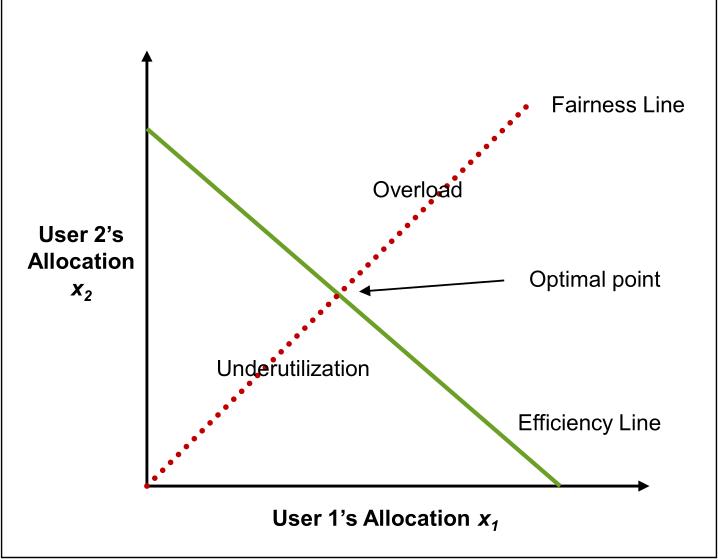
\includegraphics[width=0.5\linewidth]{./assets/util_graph.png}
   \caption{Utilization graph}%
   \label{fig:}
 \end{figure}

 A good congestion control system would move towards the optimal point. Consider an AIAD (Additive Increase, Additive Decrease) scheme. Then, both $X_1$ and $X_2$ increase and decrease by the same amount over time. If you use a policy where you increase both user's allocations by the same amount, then the point moves along a $45^{\circ}$ line, not towards the optimal point.

 If we use an MIMD scheme, both $X_1$ and $X_2$ increase or decrease by the same factor over time. This is equivalent to a point extending from origin. As this movement happens, fairness remains constant.

 Now we can see why TCP chose an AIMD model - it moves towards the optimal point. During the increase, the point moves along a $45^{\circ}$, and during the decrease the point moves towards the origin. This will eventually converge to the fairness optimal point.

\subsection{TCP Modelling}

Given the congestion control behaviour of TCP, a TCP model predicts our performance. The factors it needs to take into account are:
\begin{itemize}
  \item \textbf{Loss rate} : This affects how often the window is reduced
  \item \textbf{RTT} : This affects the rate of increase.
  \item \textbf{RTO} : This affects performance during loss recovery (what is it?)
  \item \textbf{MSS} : This affects the rate of increase of the congestion window
\end{itemize}

One such model is the \textbf{Simple TCP Model}. We assume that the RTT remains fixed, and we do not receive any delayed ACKs. Then when in steady state, the TCP loses a packet each time the window reaches $W$ packets, and drops to $W/2$ packets. In each RTT, the window will increase by 1 packet, so $W/2 \times RTT$ time will pass before the next loss. This gives us an estimation of the loss rate - the number of segments transferred would be equal to:
\[\frac{0.75 W}{RTT} \times \frac{W \cdot RTT}{2} = \frac{3W^2}{8}\]
This gives us a loss rate :
\[L = \frac{8}{3W^2}\]
\[W = \sqrt{\frac{8}{3L}}\]
Finally, we can calculate the desired bandwidth:
\begin{align*}
  R &= \frac{0.75 \cdot MSS \cdot W}{RTT} \\
  R &= \frac{MSS}{RTT \sqrt{\frac{2L}{3}}} \\
  R &= \frac{1.22 \times MSS}{RTT \sqrt{L}}
\end{align*}

\subsection{Silly Window Syndrome}

TODO

\subsection{TCP Fairness}

The goal of fairness is that if $K$ TCP sessions share some bottleneck link of bandwidth $R$, each should have average rate of $R/K$. 

TCP congestion control is desirable in many application but not in multimedia applications like streaming. They do not want their transmission rate throttled even if the network is congested. Instead, the use UDP, so that they can pump their audio and video at a constant rate and occasionally lose some packets. In doing so, they are not acting ``fair'', since they do not cooperate with other connections to adjust the transmission rate accordingly. This allows UDP sources to crowd out TCP traffic on a bottleneck link. Currently, research is being done into ways to prevent UDP traffic from lowering the Internet's throughput.

Even if we somehow were to make UDP fair, we cannot stop a TCP based application from running parallel TCP connections. Parallel TCP connections are, for example,  used to transfer multiple objects for a Web page. When an application does this, it gets a larger fraction of the bandwidth in the congested link, which is unfair to the other users of the bottleneck link.

Finally, TCP is not fair in cases when the end hosts sharing a bottleneck link have different RTTs. When multiple connections share a bottleneck link, the sessions with smaller RTT are able to grab the available bandwidth in the link more quickly, and thus enjoy higher throughputs.

\subsection{Compound TCP}

Compound TCP is an algorithm designed by Microsoft that is designed to aggressively adjust the sender's congestion window to optimize TCP for connections with large bandwidth delay products, while trying not to harm fairness. It makes congestion decisions that reduces the transmission rate based on RTT variations.

In addition to the normal congestion window, Compound TCP also maintains a delay based window \texttt{dwnd}. Then, the sender's window is given by:
\[Win = \min\{cwnd+dwnd, awnd\}\]

When the delay is small, the delay based window increases rapidly. When queueing is experienced, the delay window gradually decreases. The aim is to keep the sum of \texttt{cwnd} and \texttt{dwnd} approximately constant, equivalent to the bandwidth-delay product of the system.

\subsection{Cubic TCP}

Cubic TCP is a network congestion avoidance algorithm which can achieve high bandwidth connections over networks more quickly and reliably in the face of high latency. 

Cubic TCP is actually real-time dependent, not RTT dependent. The following variables are defined:

\begin{itemize}
  \item $\beta$, the multiplicative decrease factor
  \item $w_{max}$, the window size before last reduction
  \item $T$, the tie elapsed since the last window reduction
  \item $C$, a scaling constant,
  \item $cwnd$, the current congestion window
\end{itemize}

The standard dictates that $\beta = 0.7, C = 0.4$. Then $cwnd$ is modelled by:
\[cwnd = C(T-K)^3 + w_{max}\]
\[K = \sqrt[3]{\frac{w_{max} (1 - \beta)}{C}}\]

\chapter{Network Layer}

\section{Forwarding and Routing} 

The role of the network layer is to move packets from a sending host to a receiving host. To do so, it performs two important network layer functions:

\begin{itemize}
  \item \textbf{Forwarding:} When a packet arrives at a router's input link, it must move the packet to the appropriate output link.

  \item \textbf{Routing:} The network layer must determine the route or path taken by packets as they flow from a sender to a receiver. This is done by specific routing algorithms.
\end{itemize}

The routers contain \textbf{forwarding tables}. It is a lookup table that decides which output link interface to use depending on the destination address. This is usually done in ranges - 0 to $r_1$ will be sent on link interface 0, $r_1$ to $r_2$ will be sent on link interface 1, and so on. So that we need not have a table of size $2^{32}$, we instead use \textbf{prefix matching}. For every link interface, we store a prefix of the minimum address that would use the link interface. The length of the prefix is the minimum necessary to differentiate between entries. In case there is more than one match, we use the longest prefix matching rule.

\section{IP Addressing}

The boundary between a host and a physical link is called an \textbf{interface}. An end host would only have one interface, but a router would necessarily have more than one interface.

An IP address is associated with a single interface. In IPv4, it is 32 bits long, and hence has $2^{32}$ unique values. We generally write them in dotted decimal notation, in which each byte is written in it's decimal form and then separated by a dot from the other bytes.

The IP address number is not meaningless. To know that it means, we need to understand \textbf{subnets}. Say we had a network of multiple endhosts and routers. Then, we could detach each interface from it's host or router(imagine the device was deleted but the interfaces remained), creating islands of isolated networks, with interfaces terminating the endpoints of the isolated networks. Each of these isolated networks form a subnet.

IP addressing assigns an address to each subnet. An example is 223.1.1.0/24. The /24 notation, called the \textbf{subnet mask} indicates that the leftmost 24 bits of the 32 bit quantity identify the subnet address. This is known as the \textbf{CIDR} notation. The leftover bits identify a machine in the subnet. If the leftover bits are $000...$, then it is called the \textbf{network address} , and if the leftover bits are $111...$ then it is called the \textbf{broadcast address}. The broadcast address forwards a datagram to all hosts on the same subnet. These addresses are generally not given to any machines.

An organization is typically given a block of contiguous addresses with the same subnet prefix. The remaining bits can distinguish among devices within the same organization, and may have an additional subnetting structure.

Let us say that an ISP connects 8 different organizations. Something special about the subnetting structure we have described till now is that the ISP will only advertise that it services datagrams whose first 20 address bits match (say) 200.23.16.0/20. The rest of the world does not know that there are 8 organizations under the ISP with their own subnets. This is referred to as \textbf{address aggregation}. 

What would happen if an organization is moved to a different ISP? Would it's subnet would need to be changed? The answer is no. The new ISP could advertise multiple subnets - it's original one as well as 200.23.18.0/23 for the newly added organization.

\section{The Router}

The router has 4 high level components:

\begin{itemize}
  \item \textbf{Input ports} : The input payer is a physical endpoint terminating the incoming physical link. It also performs link layer functions, to interoperate with the link layer on the other side of the incoming link. The \textbf{lookup function}  is also performed at the input port. The forwarding table is consulted to determine the router output port to which a packet should be sent. If the switching fabric is already in use, the packets will be queued at the input port, awaiting transmission.
  \item \textbf{Switching Fabric} : It connects the input ports to the output ports. The rate at which packets can be transferred from input port to output port is called the \textbf{switching rate}. If there are $N$ inputs, we desire that the switching rate is at least $N$ times the line rate. There are three ways to perform switching:
    \begin{itemize}
      \item Switching via memory. Here routers are traditional computers, where switching is done under the direct control of the routing processor, It worked much like an operating system, with the input ports generating interrupts to perform the necessary operations.
      \item Switching via a bus. Here the input port directly transfers a packet to the output port via a shared bus, without intervention by the routing processor. The packet is prepended with a header and sent to the bus. All the output ports will receive the packet but only the one mentioned in the header will recognize it and act accordingly. Here the router switching speed is limited by the bus speed. If multiple packets arrive to the router at the same time, they must go to the bus in a queue since only one packet can use the bus at a time.
      \item Switching via an interconnection network. This is a more sophisticated network using a crossbar switch. A crossbar switch consists of $2N$ buses that connect $N$ input ports and $N$ output ports. Each of the input buses intersect with all the output buses, and can be opened or closed at any time by the switching fabric.
    \end{itemize}
  \item \textbf{Output Ports} : It stores packets received by the switching fabric and transmits these on the outgoing link by performing the necessary link layer and physical layer functions.
  \item \textbf{Routing Processor}  : The routing processor executes the routing protocols, maintains the routing tables and computes the forwarding table. Shadow copies of the forwarding tables are stored in every input port.
\end{itemize}


\section{DHCP Protocol}

How does an end host get an IP address? One way is for the IP address to be hard coded by the system administrator in some file. Another way is to use \textbf{Dynamic Host Configuration Protocol}  to dynamically get the IP address from a server. The host works as a client, and is provided an IP address by the DHCP server. This is useful when hosts are only connected intermittently.

When the DHCP server gives the host an IP address, it gives it a ``lease'', meaning that it is valid only for a specific amount of time. This lease can be renewed when necessary. The DHCP server allows for reuse of addresses, i.e. if one host leaves then another host can use it's IP address.

A DHCP server provides IP addresses for a specific subnet. Having one DHCP server for every subnet is very wasteful. Hence, the router will have a ``relay agent'', which will forward the DHCP messages from the hosts to an appropriate DHCP server.

The protocol works as follows:

\begin{enumerate}
  \item The client sends a ``DHCP discover'' message, which is a broadcast message looking for a DHCP server. The \texttt{src} field will hold IP address 0.0.0.0, since no IP address has been given. The \texttt{dest} field will hold the IP address 255.255.255.255, since the message is being broadcast. Every message also has a transaction ID, to keep track of the messages.
  \item The server responds with a ``DHCP offer''. The \texttt{src} field will hold the IP address of the DHCP server, and the \texttt{dest} field will once again have the broadcast IP address. It will also have a field \texttt{yiaddrr} holding the leased IP address, and a field \texttt{lifetime} for the tie of the lease. Of course, it will also have the same transaction ID as the discover message.
  \item The client will respond with a ``DHCP request''. It needs to respond again because the client may receive multiple DHCP offers, and hence the server cannot immediately provide the client with an address. The client hence chooses one of the offers and responds. The request will once again have the \texttt{src} 0.0.0.0, and the broadcast destination address. Now, the transaction ID will be different. The \texttt{lifetime} and \texttt{yiaddrr} field will be the same as sent in the DHCP offer, so that the server knows who had sent it.
  \item Finally, the server sends a ``DHCP ACK''. This has the same contents as the DHCP offer, but with the same transaction ID as in the request. After receiving this, the client assumes the given IP address.
\end{enumerate}

\section{The IP Datagram}

The key field of IPv4 datagram are:

\begin{itemize}
  \item \textbf{Version Number} : This 4 bit  field specify the IP protocol version of the datagram
  \item \textbf{Header Length}  : Since the IPv4 datagram can contain a variable number of options, these 4 bits are needed to determine where the IP datagram data actually begins.
  \item \textbf{Type of Service} : The type of service bits were included in the IPv4 header to allow different types of IP datagrams to be distinguished from each other. For instance, we may want to distinguish between real time and non real time traffic
  \item \textbf{Datagram length}  : The total length of the IP datagram (header + datae) measured in bytes. It is a 16 bit field.
  \item \textbf{Identifiers, flags, and fragmentation offset} : These three fields have to do with fragmentation
  \item \textbf{Time to live} : The TTL field is included to ensure that datagrams do not circulate forever. This field is decremented by one each time the datagram is processed by a router. If the TTL field reaches 0, the datagram must be dropped.
  \item \textbf{Protocol} : This field is used only when an IP datagram reaches its destination, and indicates the transport layer protocol to which the data portion of the IP datagram should be passed. A value of 6 means TCP, and a value of 17 means UDP.
  \item \textbf{Header Checksum} : This allows the router to check for bit errors in the IP datagram. This is calculated by computing each 2 bytes in the header as a number and summing them all up with 1s complement arithmetic.
  \item \textbf{Source and Destination IP addresses} 
  \item \textbf{Options}  The options field allows an IP header to be extended.
  \item \textbf{Data} : The data field holds the actual payload, which could be the transport layer segment or an ICMP message.
\end{itemize} 

\section{IP Fragmentation and Reassembly}

All link layer protocols cannot carry network layer packets of the same size. The maximum amount of data that can be carried is the MTU. The problem that arises is that different links can have different MTUs, and hence may be incapable of sending some incoming datagrams.

In order to fix this issue, the IP datagram is broken up into two or more smaller IP datagrams, called \textbf{fragments}. These need to be reassembled before they reach the transport layer, since it expects complete segments form the network layer. This reassembly is done at the end hosts.

The reassembly is done using the identification, flag and fragmentation offset fields in the IP datagram header. When a datagram is created, the sending host gives the datagram a identification number. When the router fragments this datagram, the identification order remains the same for every fragment. Now when the destination receives the fragments, it can check these identification numbers to determine if the datagrams are actually fragments of the same larger datagram.

Of course, the network layer is unreliable so some datagrams may be lost. Hence, the last fragment has the flag bit set to 0, whereas all other fragments have the flag bit set to one. To piece together the fragments, we use the fragmentation offset field.

\section{Network Address Translation}

Within an organization, end hosts may have separate \textbf{private IP addresses}. These can only be used for communication within the organization. It cannot be used to interface with the Internet, since these IP addresses may not be unique.

Private address allow the local network to use just one IP address for interfacing with the internet. This allows us to change addresses of devices within the local network without notifying the outside world, or change the ISP without changing addresses of devices in the local network. Moreover, from a security perspective, the devices inside the local network are not addressable or visible to the outside world.

\begin{figure}[htpb]
  \centering
  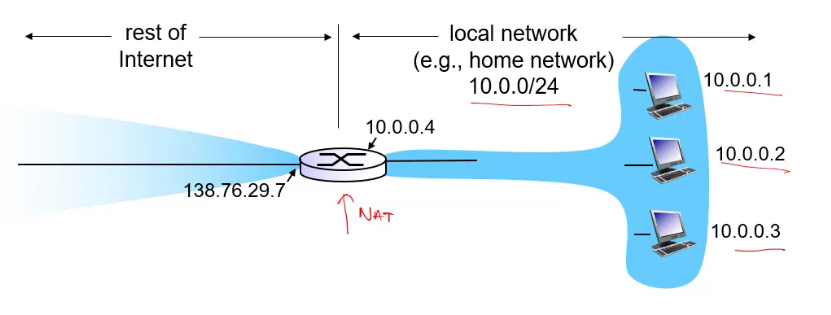
\includegraphics[width=0.8\linewidth]{./assets/NAT_eg.png}
  \caption{./assets}%
  \label{fig:./assets}
\end{figure}

In Figure 1, we can see the structure of the NAT. All datagrams leaving the local address will have the same source address (138.76.29.7), and all the datagrams coming into it will have the same destination address (138.76.29.7), since the router is the only access point to the Internet.

The router will hold a \texbf{NAT translation table}, which will map the WAN side addresses to the LAN side addresses. When (say) 10.0.0.1, 3345 sends a datagram, to (say) 128.119.40.186, 80, the NAT router will change the source address to 138.76.29.7,5001, and send it to the destination. At the same time, it will create an entry in the translation table with the WAN side address 138.76.29.7,5001 and the LAN side address 10.0.0.1,3345. When the response arrives, it will have the destination as 138.76.29.7,5001. Then, the router will check the NAT translation table and forward it to the appropriate machine and port number.

Since the 16 bit port number field is the only differentiating factor for the WAN side address, at most $2^{16}-1$ devices can be connected. NAT is also controversial since the router is checking the transport layer packet for the port number, which violates the layered architecture of the internet.

Consider a client outside the local network wants to connect to a server with address 10.0.0.1. The only visible address is the NATed address, 138.76.29.7, not the internal server address. Therefore, to address this, we need to do some special configuration:

\begin{itemize}
  \item Statically configure the NAT to forward incoming connection requests at a given port to the server.
  \item Another way is to use the Universal Plug and Play (UPnP) protocol. It learns the public IP address and can add or remove port mappings with lease times. For instance, an application can ask the NAT to create a mapping from (say) 10.0.0.1,3345 to (say) 138.76.29.7,5001. This way, the network administrator need not manually configure the NAT.
  \item The last method is to use relaying. The NATed client establishes connection to a relay. The relay then bridges packets between external clients and th NATed client. This is used in Skype.
\end{itemize}

\section{IPv6}

IPv6 is the successor to the IPv4 protocl, allowing for a larger address space as well as some other improvements.

In Fig we can see the IPv6 datagram format.

\begin{figure}[htpb]
  \centering
  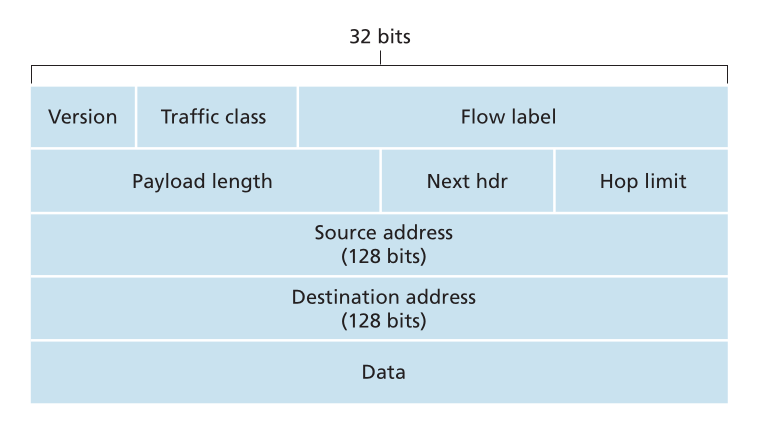
\includegraphics[width=0.8\linewidth]{./assets/ipv6_datagram.png}
  \caption{An IPv6 datagram}%
  \label{fig:}
\end{figure}

The important differences are:

\begin{itemize}
  \item The size of the IP address is now 128 bits, instead of 32.
  \item There is now an \textbf{anycast address}, that allows sending to any one of a group of hosts.
  \item The header length is a fixed 40 bits in size
  \item IPv6 allows for flow labelling. This allows for the labelling of packets belonging to particular flows to handle them specially. For instance, audio or video transmission could be treated as flows.
\end{itemize}

The fields are:
\begin{itemize}
  \item \textbf{Version}, holding the value 6 for IPv6
  \item The \textbf{traffic class} is an 8 bit field similiar to the TOS field in the IPv4 datagram
  \item The \textbf{flow label} is used for identifying flow datagrams
  \item The \textbf{payload length}  is the number of bytes in the datagram that follow the header.
  \item \textbf{Next Header}  identifies the protocol to which to deliver the datagram
  \item The \textbf{Hop limit}  is the same as TTL in the IPv4 datagram
  \item The source and destination addresses
  \item The actual payload
\end{itemize}

IPv6 does not allow for fragmentation and reassembly at intermediate routers. Instead, this is only done by the source and destination. If the datagram is too large for a router, it answers with a ``Packet Too Big"" ICMP error message. This speeds up IP forwarding within the network.

It is also noticeable that there is no longer a header check sum. This is because the transport and link layers both perform checksumming, so it was removed in IPv6 in the interest of speed.

Given these technical details, how do we transition from IPv4 to IPv6? It is clearly impossible to coordinate a mass upgrade from old IPv4 systems to the new IPv6, considering the size of the internet today. Instead we use a \textbf{dual stack} approach, where IPv6 nodes also have a complete IPv4 implementation. These have the ability to send and receive both IPv4 and IPv6 datagrams, and have both kinds of addresses. 

These dual stack nodes have to be capable of checking whether or not the next node is IPv6 compatible. To do this, we can use DNS - if the node name is resolved to have an IPv6 address, it must be IPv6 compatible. Otherwise, it is IPv4-only.

This dual stack approach faces a huge issue. Consider an example where Alice and Bob both have IPv6 compatible machines, and want to communicate with one another. But one of the nodes on the path between them is IPv4-only. In this case, the IPv6 datagrams sent by Alice would have to be converted to IPv4. Unfortunately, there are field in the IPv6 datagrams that have no counterpart in IPv4, so that information is lost.

An alternative is \textbf{tunnelling}. We refer to the set of IPv4 nodes as a \textbf{tunnel}. The IPv6 node on one side of a tunnel takes the entire IPv6 datagram and puts it in the data field of an IPv4 datagram. The IPv4 datagram received on the other side of the tunnel can be used to extract the IPv6 datagram and route as normal.

\section{ICMP}

ICMP stands for the Internet Control Message Protocol. ICMP is used by hosts and routers to communicate network layer information with one another. For instance, a popular use of ICMP is for error reporting.

ICMP messages are carried inside the IP datagram payload, just like transport layer segments. When a host receives an IP datagram with ICMP specified as the upper layer protocol, it demultiplexes the contents to ICMP, just like with the transport layer protocols.

Every ICMP message has a \texttt{type} and a \texttt{code} field, and contains the header and the first 8 bytes of the IP datagram that caused the ICMP message to be generated. This way the sender can determine the datagram that caused the error.

Some important examples of ICMP messages are ``Destination Unreachable'', ``source quench'' (used for congestion control), ``echo reply'' (used to ping).

\section{Routing Algorithms}

\subsection{The Terminology}

Typically, a host is attached directly to one router which is called the \textbf{default router} . The default router connected to the source host is called the \textbf{source router}. Hence the problem of routing a packet from source host to the destination hos boils down to the routing of a packet from the source router to a destination router.

Routing algorithms can be of many (not necessarily exclusive) types:
\begin{itemize}
  \item \textbf{Global}, where each node has complete information about connectivity and link costs
  \item \textbf{Decentralized}, where each node begins with only the knowledge of the costs of its own directly attached links. Then, it uses an iterative process of calculation to find the least cost paths.
  \item \textbf{Static}, where routes change very slowly over time
  \item \textbf{Dynamic}, where routes change due to the traffic load or change in topology
  \item \textbf{Load sensitive}, where link cost changes due to congestion in the link
  \item \textbf{Load insensitive} , where link costs do not change with congestion
\end{itemize}

\subsection{Link State Routing Algorithms}

LS algorithms are global algorithms - they have complete information about the network topology and all link costs. This is done in practice via link state broadcast algorithms, where each node broadcasts to all the other nodes on the network.

One LD algorithm is Djikstra's algorithm, which can compute all least-cost paths from a source node $u$ to all the other nodes. After the $k^{th}$ iteration, the least cost paths are known to $k$ destination nodes. The algorithm is well known, but remember the following notation:
\begin{itemize}
  \item $D(v)$ - the cost of the least cost path from $u$ to $v$
  \item $p(v)$ the predecessor on the least cost path
  \item $N'$ the subset of nodes, where $v$ is in $N'$ if the least cost path is known.
\end{itemize}

In $O(n \log n)$ (in sparse graphs) time, we can fill the forwarding table with information of the next-hop node on the least cost path from $u$ to it's destination.

This approach can lead to some problems - assume that the link costs are equivalent to the load on the link. In this example, link costs are not symmetric. This means we are now trying congestion-sensitive routing. In this case, there may be \textbf{route oscillations}, where the route changes with new costs on every timestep.

\textbf{TODO : OSPF}

\subsection{Distance Vector Routing Algorithm}

While the LS algorithm us an algorithm using global information, the DV algorithm is iterative, asynchronous and distributed. This means that each node receives some information from one or more of its directly attached neighbours, performs a calculation, and then distributes the results of its calculation back to its neighbours.

The DV algorithm is governed by the \textbf{Bellman Ford Algorithm}, given by:
\[d_x (y) = \min_v \{c(x,v) + d_v(y)\}\]
Each node $x$ begins with $D_x(y)$, an estimate of the cost of the least cost path form itself to node $y$, for all nodes in $N$. Let $\mathbf{D}_x = [D_x(y) : y \in N]$ be the distance vector for node $x$. With the DV algorithm, each node $x$ maintains the following information:
\begin{itemize}
  \item For each neighbour $v$, the cost $c(x,v)$ from $x$ to directly attached neighbour $v$
  \item Node $x$ distance vector $\mathbf{D}_x$
  \item The distance vectors of each of it's neighbours $\mathbf{D}_v$
\end{itemize}
From time to time, each node sends a copy of its distance vector to each of its neighbours. When $x$ receives a new distance vector from $v$, it saves $\mathbf{D}_v$, and then uses the Bellman Ford equation to update it's own distance vector.
If node $x$'s distance vector has changed, then it will send its updated distance vector to each of its neighbours. It can be proved that this will eventually converge to the actual cost of the least cost path.

Though we can be sure that the distances will eventually converge, how long can it take to converge? Consider the network given in Fig. 5.3.

\begin{figure}[htpb]
  \centering
  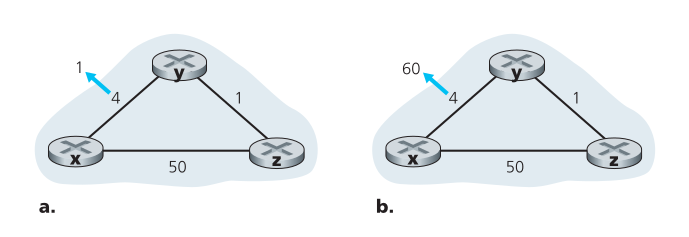
\includegraphics[width=0.8\linewidth]{./assets/dv_eg.png}
  \caption{Routing network example}%
  \label{fig:}
\end{figure}

If, like in example (a), we reduce the link cost from 4 to 1, what will happen? Let us consider the distance table entries of $y$ and $z$ to $x$. First, $y$ will notice the link cost change, change the distance vector and send it to $z$. $z$ will then update it's own distance vector (since the minimum cost is now 2) and notify $y$ of this. $y$ will not make any changes, so the process stops here. We only needed 2 iterations.

But what about in example (b)? The link cost changed from 4 to 60. $y$ will detect this, and compute a new minimum cost path to $x$ as:
\[D_y(x) = min \{c(y,x) + D_x(x), c(y,z) + D_z(x)\} = \min \{60 + 0, 1 + 5\} = 6\]
This is, of course wrong, but nevertheless, $y$ will do this. Now, $y$ will route through $z$ to get to $x$, but $z$ will want to route to $y$ to get to $x$. This forms a \textbf{routing loop}, which will keep bouncing packets between $y$ and $z$ till there is a change in the routing table. $y$ will inform $z$ of the change, and $z$ will update it's own least cost to $D_z(x) = 7$. Then it will inform $y$ of this. It will take 44 iterations to find out the actual correct routing table.

This presents a big problem. What if we changed to some very large value? It would take a long time to fix the routing loop. This is called the \textbf{count-to-infinity problem}.

This can be fixed with some modifications. One such rule is the \textbf{poison reverse rule} , which states that routes received via one interface have to be advertised back out from that interface with an unreachable metric. That means that if $z$ routes through $y$ to get to $x$, then $z$ will advertise to $y$ that its distance to $x$ is infinity. This will remove the routing loop, since $y$ will never attempt to route to $x$ via $z$, as long as $z$ continues to route to $x$ via $y$.

Another rule is the \textbf{split horizon rule}  that states that a route can't be advertised out of the interface if the next hop for the advertised route is found on that interface.

\section{Routing Information Protocol}

The RIP is a protocol for routing within an \textbf{autonomous system} (AS). An autonomous system is a group of routers that are typically under the same administrative control. Routers in the same AS use the same routing algorithm and have information about one another. Since RIP is for routing within an autonomous system, it is called a \textbf{intra-AS routing protocol}.

The RIP is a DV protocol that uses the hop count as a cost metric - this means that every link has a cost of 1. In RIP, the costs are from the source router to a destination subnet. This is unlike the DV protocol previously discussed, where the costs where defined between routers. Hence, a hop is now defined as the number of subnets on the path from the source router to the destination subnet.

The maximum cost of a path is limited to 15, hence limiting the size of the network admissible for using the RIP protocol.  In RIP, routing updates are exchanged between neighbours approximately every 30 seconds using \textbf{RIP response messages}. The response message contains a list of up to 25 destination subnets within the AS, as well as the sender's distance to each of those subnets. They are sent as UDP packets, and periodically repeated.

Each router maintains a routing table called the \textbf{RIP table}. This contains both the distance vector and the forwarding table. The table has 3 columns - one for the destination subnet, another for the next router, and the last for the number of hops.





\chapter{Data Link Layer}

\section{Introduction}

The Data Link Layer uses the services of the Physical layer to deliver link-layer packets, which are called \textbf{frames}.


\end{document}
